%\section{Evaluation}
%%%% ASLAK: Start by explaining why these areas are: 1. important 2. covers what is important
In our project we have two areas that we have been evaluating. The first being wheter our policy engine is actually working and enforcing the defined policies. The other being the front-end interface, testing to uncover potential usability issues that needed solving.
This is important as we need to see how well our system performs and to see what has been implemented from the requirements.
\section{Policy Engine System Evaluation}
\label{policy-engine-system-evaluation}

\subsection{Log Testing}
\label{log-test}
We have logged system data which was important as to determine if the system is working correctly. Doing so we have been able to verify the results and outcome while testing and to discover bugs in our implementation.
For quality control we have also been using these log files. Verifying our solution by cross-referencing every action during tests, and match it with the actual data stored in the database.
One excerpt from the log file can be seen in figure \ref{fig:log}

\begin{figure}[ht]
\centering
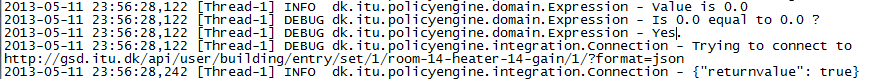
\includegraphics[width=\columnwidth]{images/logoutput.png}
\caption{An excerpt from the log file.}
\label{fig:log}
\end{figure}

\subsection{JUnit Testing}
To further test the software we made, we performed a range of JUnit Tests. After the creation of the domain classes we have created JUnit test to verify if everything works as expected. 
One example of these test can be seen in \ref{appendix:junit-test}. In this test we set the temperature of a room to 11 degrees and we want to turn on the heater in the room if the temperature is equal to 10 degrees, otherwise we want to roll down the blinds. The test will succed when checking if the blinds are rolled down, as the temperature is set to 11 degrees. 
We have employed tests for checking all the posibilities of operations against the operators. 
The result was that our IF-THEN-ELSE concept implementation performed as expected. 
%%Rasmus: jUnit test reference is missing

\section{Usability Test}
\label{sec:usability-test}
To evaluate on the usability of our policy engine we decided to make a test with candidates outside of our development group.

In general, when it come to "best practices of usability tests", the Think Aloud Protocol is considered one of the most valuable \cite{Nielsen1993}.

Therefore we decided to use it for our evaluation. Also the Think Aloud Protocol, is inexpensive in cost and time, and it is easy to set up and gives very valuable result from real-life scenarios. 

\subsection{Think Aloud Protocol}
In a thinking aloud test, you ask test participants to use the system while continuously thinking out loud — that is. Simply verbalizing their thoughts as they move through the user interface, and take actions.

To run a basic thinking aloud usability study, 3 things is required:
\begin{itemize}
\item Recruit representative users.
\item Inform them of representative tasks to perform. %%ASLAK: Perhaps someone from FM??
\item Avoid interference and let the users speak their actions.
\end{itemize}

We invited five people to a think aloud test. Research shows that having just five people will potentially uncover 80\% of all usability problems \cite{jakobnielsen2000fiveusers} as seen on \ref{fig:usabilitycurve}.

\begin{figure}[ht]
\centering
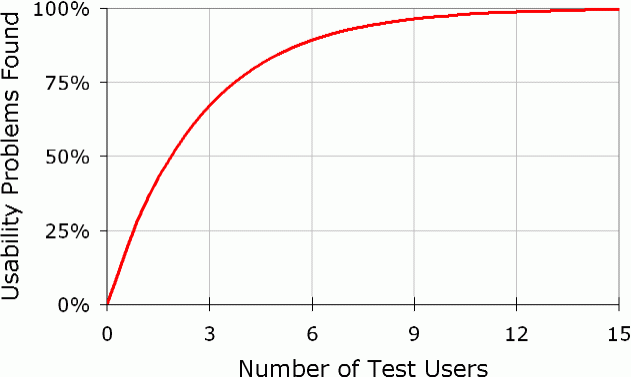
\includegraphics[width=\columnwidth]{usabilitycurve.png}
\caption{Usability test graph.}
\label{fig:usabilitycurve}
\end{figure}

The candidates is male and female students at ITU, between the age of 25 and 30. Some of them study software development and have a lot of knowledge in programming, others study digital design and knows more about human computer interaction and usability. However they all have web development in common.

\subsubsection{Tasks}
We arranged 7 tasks for the candidates to perform.  Note however that the tests where held individually from each candidate, but they were all giving the same set of tasks. 
During the tests, candidates where only given one tasks at a time to focus on - using small tasks cards.

The candidates where assigned the following tasks. The questions is designed so that the candidates makes use of all the features in policy engine:

Before the test started we explained the purpose of the Policy Engine, and verbally gave them an example of a user case scenario.
We briefly introduced the participant with a map of the building and the rooms involved. We also gave an example list of sensor and actuator -names to get them familiar with the elements involved including basic knowledge of IF, AND, THEN statements and wild card operators.

Note that the user interface is designed with "live auto complete functions" so that the user can easily set a desired sensor/actuator without knowing the exact name. See section \ref{managing-policies} for more details.

\begin{framed}
Create a policy that turns the AC on in Room 1, 1. floor and name it "Cooling".
\end{framed}
The first task is designed to see how the user is creating new policy - including the use of naming the individual policies.

\begin{framed}
Modify the "Cooling" policy you just created to affect both Room 1, 1. floor and Room 2, 2. floor.
\end{framed}
The second task is designed to see how the user handles modifying a policy.

\begin{framed}
Create a policy that turns on Blinds in all rooms for every floor in the building and name the policy "Sun".
\end{framed}
The third task is designed to see how the participant handles the "wildcard" feature.

\begin{framed}
Find and show the active policies just created.
\end{framed}
This furth task shows how well the user handles listing active policies. As this would likely be a typical task for a building administrator.

\begin{framed}
Disable the policy named "Cooling" so that is no longer in function.
\end{framed}
The fifth task shows how well the user handle disabling/activating policies.

\begin{framed}
Delete the policy named "Sun".
\end{framed}
The sixth tasks shows the removal of policies.

\begin{framed}
To save energy the university wants to have the heating turned OFF automatically at 17:00. However this Wednesday around 19:00 - 22:00 an exclusive presentation is held in room number 5 on 1. floor.
You are asked to maintain a temperature at 21 degrees in that room throughout the presentation.
\end{framed}
The seventh task is designed to be more complex and the user is forced to work with expressions (AND) and operators such as larger than (\textgreater).


\begin{framed}
It is summertime and the overall temperature inside the building is rising. You are asked to keep temperature at maximum 22 in all of the rooms in the building.
\end{framed}
The eigth task is designed to be 


\begin{framed}
All afternoon between 12:00 and 16:00 the sun is at its peak. Therefore you are asked to set blinds ON in all the rooms on 1. floor and 2. floor - but only if the lights are ON.
\end{framed}

\begin{framed}
The university wants to save energy. You are asked to make sure lights are automatic turned OFF at 17:00 in all the rooms, except from those on 0. Floor.
\end{framed}



\subsubsection{Results and Comments}
\label{results-and-comments}
After every participant had gone through the think aloud test. We went through all their remarks. Some were the same, and those that were - we combined into one.
For all the remarks, we made some comments as listed below - including the actions we took to further improve the software.

\begin{quotation}
If there is a lot of policies - which I would expect there will be? Then I think the active policy list will be too long. I think it would make it difficult to find a specific (policy) if say you have a 100 policies.
\end{quotation}

The user is referring to the “Active Policy Site”, from which every active policy is listed underneath each other. The user finds that the site may force the user to do a lot of scrolling in order to find a specific policy.

Due to this we implemented a expand function, which instead of listing all the content, in all of the listed policy. It on shows name and time and a button in the right hand corner, which if clicked expands the policy and reveals all of the content. This way the list will be much more compact and easier to go through. 

For future implementation we would also like to make a search function, from which the user is able to filter the policy by the search inputs. In example: name, or rooms effected  by the policy etc.
 
\begin{quotation}
I think it is difficult to see which one (rules) belong to what (expression).
\end{quotation}

The user is referring to the rules within a given policy. In every policy the user have the option to use expressions such as IF, THEN, ELSE. The user finds that it is difficult to see which rules belong to what expression (IF, THEN and ELSE).

Due to this we implemented a color technique, which colorize the rules that belongs under the same expression. As an example all the rules belonging to an IF -expressions is colored with a red background on the site, while all the THEN –expression is colored green.

In the second think aloud test, all participant expressed that they loved the coloring. That they diffidently feel that the overview is much better and think it is easier to understand.

\subsubsection{Subset}
After the first think aloud test, we made changes to front-end design and we repeated the think aloud test, using the same set of tasks, to verify the improvements. 

After the second round of testing we only had some minor changes to do. But overall the participant where comfortable with usability and had no further remarks.
We believe that there is always room for improvement. And so we have made some comments on this in section \ref{subsec:improvements}.
 

%ATTENTION: Note: Insert results from think aloud test and write what we have learned from this


